\chapter{Proposed Work}
\label{chap:proposed.work}

\section{Truncated Bayes by Backprop Through Time}
\label{sec:tbbbtt}

Applying BBB to RNNs is depicted in Figure \ref{fig:lstmbbb} where the weight matrices of the RNN are drawn from a distribution (learnt by BBB).
However, this direct application raises two questions: when to sample the parameters of the RNN, and how to weight the contribution of the KL regulariser of \eqref{eq:klelbo}.
We shall briefly justify the adaptation of BBB to RNNs, given in Algorithm~\ref{alg:rnnbbb} below.

\begin{figure}
	\centering
	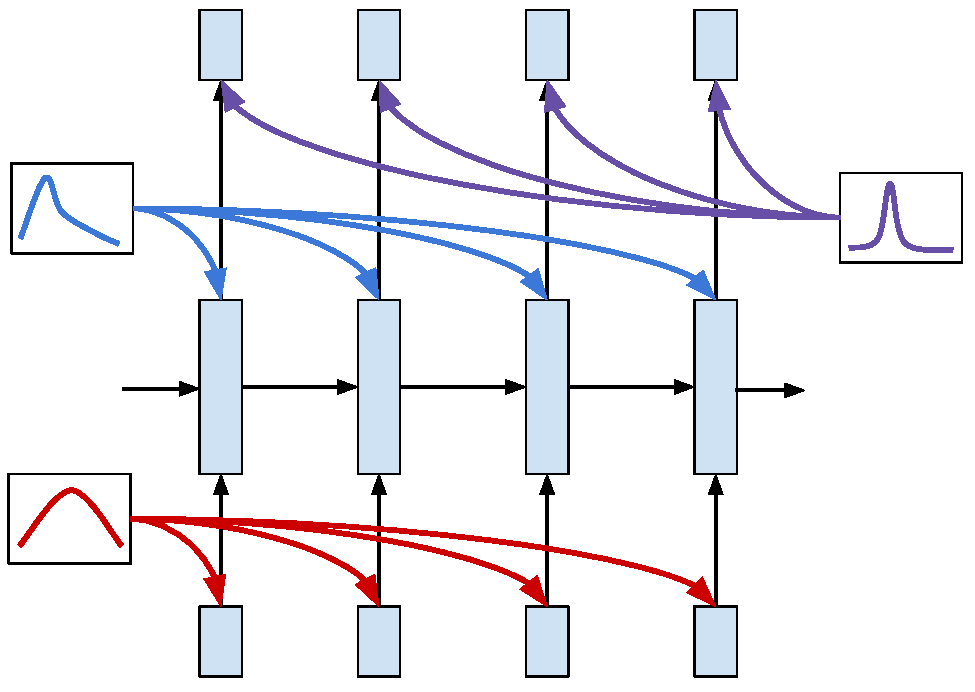
\includegraphics[width=\linewidth]{figs/LSTMBBB}
	\caption{Demonstration of Bayes by Backprop (BBB) applied to an RNN.}
	\label{fig:lstmbbb}
\end{figure}

The variational free energy of \eqref{eq:klelbo} for an RNN on a sequence of length $T$ is:
\begin{align}
	\mathcal{L}(\theta) &=
	- \mathbb{E}_{q(\theta)}\left[\log p(y_{1:T}|\theta, x_{1:T}) \right]
	\nonumber \\
	&\phantom{=}
	+ \kl{q(\theta)}{p(\theta)},
	\label{eq:rnnelbo}
\end{align}
where $p(y_{1:T}|\theta, x_{1:T})$ is the likelihood of a sequence produced when the states of an unrolled RNN $F_T$ are fed into an appropriate probability distribution.
The parameters of the entire network are $\theta$.
Although the RNN is unrolled $T$ times, each weight is penalised just once by the KL term, rather than $T$ times.
Also clear from \eqref{eq:rnnelbo} is that when a Monte Carlo approximation is taken to the expectation, the parameters $\theta$ should be held fixed throughout the entire sequence.

Two complications arise to the above naive derivation in practice: firstly, sequences are often long enough and models sufficiently large, that unrolling the RNN for the whole sequence is prohibitive.
Secondly, to reduce variance in the gradients, more than one sequence is trained at a time.
Thus the typical regime for training RNNs involves training on mini-batches of truncated sequences.

Let $B$ be the number of mini-batches and $C$ the number of truncated sequences (``cuts''),
then we can write \eqref{eq:rnnelbo} as:
\begin{align}
	\mathcal{L}(\theta) &=
	- \mathbb{E}_{q(\theta)}\left[\log \prod_{b=1}^B \prod_{c=1}^{C} p(y^{(b,c)}|\theta, x^{(b,c)}) \right]
	\nonumber \\
	&\phantom{=}
	+ \kl{q(\theta)}{p(\theta)},
\end{align}
where the $(b,c)$ superscript denotes elements of $c$th truncated sequence in the $b$th minibatch.
Thus the free energy of mini-batch $b$ of a truncated sequence $c$ can be written as:
\begin{align}
	\mathcal{L}_{(b,c)}(\theta) &=
	- \mathbb{E}_{q(\theta)}\left[\log p(y^{(b,c)}|\theta, x^{(b,c)}, s^{(b,c)}_\text{prev}) \right]
	\nonumber \\
	&\phantom{=}
	+ w^{(b,c)}_\text{KL} \kl{q(\theta)}{p(\theta)},
	\label{eq:weightelbo}
\end{align}
where $w^{(b,c)}_\text{KL}$ distributes the responsibility of the KL cost among minibatches and truncated sequences (thus $\sum_{b=1}^B \sum_{c=1}^C w^{(b,c)}_\text{KL} = 1$), and $s^{(b,c)}_\text{prev}$ refers to the initial state of the RNN for the minibatch $x^{(b,c)}$.
In practice, we pick $w^{(b,c)}_\text{KL} = \frac{1}{C B}$ so that the KL penalty is equally distributed among all mini-batches and truncated sequences.
The truncated sequences in each subsequent mini-batches are picked in order, and so $s^{(b,c)}_\text{prev}$ is set to the last state of the RNN for $x^{(b,c-1)}$.

Finally, the question of when to sample weights follows naturally from taking a Monte Carlo approximations to \eqref{eq:weightelbo}: for each minibatch, sample a fresh set of parameters.

\begin{algorithm}[ht]
	\caption{Bayes by Backprop for RNNs}
	\label{alg:rnnbbb}
	\begin{algorithmic}
		\STATE{Sample $\epsilon \sim \mathcal{N}(0,I)$, $\epsilon \in \mathbb{R}^d$.}
		\STATE{Set network parameters to $\theta = \mu + \sigma\epsilon$.}
		\STATE{Sample a minibatch of truncated sequences $(x,y)$.}
		\STATE{Do forward propagation and backpropagation as normal on minibatch.}
		\STATE{Let $g$ be the gradient with respect to $\theta$ from backpropagation.}
		\STATE{Let $g^{KL}_\theta, g^{KL}_\mu, g^{KL}_\sigma$ be the gradients of $\log \mathcal{N}(\theta|\mu, \sigma) - \log p(\theta)$ w.r.t. $\theta$, $\mu$ and $\sigma$ respectively.}
		\STATE{Update $\mu$ according to the gradient $\frac{g + \frac{1}{C}g^{KL}_\theta}{B} + \frac{g^{KL}_\mu}{B C}$.}
		\STATE{Update $\sigma$ according to the gradient $\left(\frac{g + \frac{1}{C} g^{KL}_\theta}{B}\right) \epsilon + \frac{g^{KL}_\sigma}{B C}$.}
	\end{algorithmic}
\end{algorithm}

\section{Analytical Proofs}


\section{Results and Discussion}


\begin{table}[p]
	\centering
	\caption[Short version of the caption.]{Example of a table. This is a long, very long, long long, long caption.  You can give a shorter caption for the ``list of table" using the square braket symbol.}
	\vspace{\baselineskip}
	\begin{tabular}{l c c}
		\hline
		\hline
		Temperature & Resonant Frequency & Q factor\\
		\hline
		13 mK $\pm$ 1 mK & 16.93 & 811 \\
		40 mK $\pm$ 1 mK & 16.93 & 817 \\
		100 mK $\pm$ 1 mK & 16.93 & 815 \\
		300 mK $\pm$ 1 mK & 16.93 & 806\\
		500 mK $\pm$ 1 mK & 16.93 & 811\\
		800 mK $\pm$ 5 mK & 16.93 & 814\\
		1000 mK $\pm$ 5 mK & 16.93 & 806 \\
		\hline
		\hline
	\end{tabular}
\end{table}

\section{Chapter Summary}